% GENERATED by pipeline/figures/plot_planner_steps.py -- do not edit by hand.
% Regenerate after any change to raw_data/plan_sweep/ (experiments/plan_sweep/run.py).
\begingroup%
\definecolor{pink}{HTML}{1C1B18}%
\definecolor{pmid}{HTML}{6B6A65}%
\definecolor{pgrid}{HTML}{C9C7C0}%
\definecolor{pblue}{HTML}{2A78D6}%
\definecolor{porange}{HTML}{EB6834}%
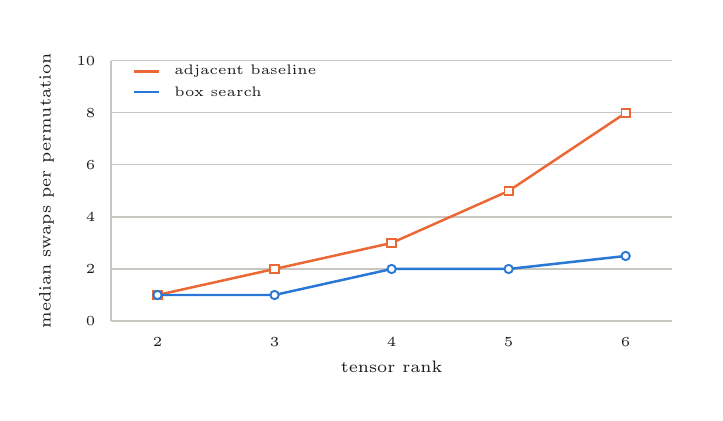
\begin{tikzpicture}[x=1pt,y=1pt]%
\useasboundingbox (0,0) rectangle (241.00,132.00);%
\draw[pgrid,line width=0.4pt] (30.00,26.00) -- (233.00,26.00);%
\node[anchor=east,text=pink,font=\fontsize{5.5}{6.5}\selectfont] at (28.00,26.00) {0};%
\draw[pgrid,line width=0.4pt] (30.00,44.80) -- (233.00,44.80);%
\node[anchor=east,text=pink,font=\fontsize{5.5}{6.5}\selectfont] at (28.00,44.80) {2};%
\draw[pgrid,line width=0.4pt] (30.00,63.60) -- (233.00,63.60);%
\node[anchor=east,text=pink,font=\fontsize{5.5}{6.5}\selectfont] at (28.00,63.60) {4};%
\draw[pgrid,line width=0.4pt] (30.00,82.40) -- (233.00,82.40);%
\node[anchor=east,text=pink,font=\fontsize{5.5}{6.5}\selectfont] at (28.00,82.40) {6};%
\draw[pgrid,line width=0.4pt] (30.00,101.20) -- (233.00,101.20);%
\node[anchor=east,text=pink,font=\fontsize{5.5}{6.5}\selectfont] at (28.00,101.20) {8};%
\draw[pgrid,line width=0.4pt] (30.00,120.00) -- (233.00,120.00);%
\node[anchor=east,text=pink,font=\fontsize{5.5}{6.5}\selectfont] at (28.00,120.00) {10};%
\node[anchor=north,text=pink,font=\fontsize{5.5}{6.5}\selectfont] at (46.92,23.50) {2};%
\node[anchor=north,text=pink,font=\fontsize{5.5}{6.5}\selectfont] at (89.21,23.50) {3};%
\node[anchor=north,text=pink,font=\fontsize{5.5}{6.5}\selectfont] at (131.50,23.50) {4};%
\node[anchor=north,text=pink,font=\fontsize{5.5}{6.5}\selectfont] at (173.79,23.50) {5};%
\node[anchor=north,text=pink,font=\fontsize{5.5}{6.5}\selectfont] at (216.08,23.50) {6};%
\draw[pgrid,line width=0.6pt] (30.00,26.00) -- (233.00,26.00);%
\draw[pgrid,line width=0.6pt] (30.00,26.00) -- (30.00,120.00);%
\draw[porange,line width=0.9pt] (46.92,35.40) -- (89.21,44.80) -- (131.50,54.20) -- (173.79,73.00) -- (216.08,101.20);%
\fill[white] (45.42,33.90) rectangle (48.42,36.90);%
\draw[porange,line width=0.7pt] (45.42,33.90) rectangle (48.42,36.90);%
\fill[white] (87.71,43.30) rectangle (90.71,46.30);%
\draw[porange,line width=0.7pt] (87.71,43.30) rectangle (90.71,46.30);%
\fill[white] (130.00,52.70) rectangle (133.00,55.70);%
\draw[porange,line width=0.7pt] (130.00,52.70) rectangle (133.00,55.70);%
\fill[white] (172.29,71.50) rectangle (175.29,74.50);%
\draw[porange,line width=0.7pt] (172.29,71.50) rectangle (175.29,74.50);%
\fill[white] (214.58,99.70) rectangle (217.58,102.70);%
\draw[porange,line width=0.7pt] (214.58,99.70) rectangle (217.58,102.70);%
\draw[pblue,line width=0.9pt] (46.92,35.40) -- (89.21,35.40) -- (131.50,44.80) -- (173.79,44.80) -- (216.08,49.50);%
\fill[white] (46.92,35.40) circle (1.5pt);%
\draw[pblue,line width=0.7pt] (46.92,35.40) circle (1.5pt);%
\fill[white] (89.21,35.40) circle (1.5pt);%
\draw[pblue,line width=0.7pt] (89.21,35.40) circle (1.5pt);%
\fill[white] (131.50,44.80) circle (1.5pt);%
\draw[pblue,line width=0.7pt] (131.50,44.80) circle (1.5pt);%
\fill[white] (173.79,44.80) circle (1.5pt);%
\draw[pblue,line width=0.7pt] (173.79,44.80) circle (1.5pt);%
\fill[white] (216.08,49.50) circle (1.5pt);%
\draw[pblue,line width=0.7pt] (216.08,49.50) circle (1.5pt);%
\node[anchor=north,text=pink,font=\fontsize{6}{7}\selectfont] at (131.50,15.00) {tensor rank};%
\node[anchor=south,rotate=90,text=pink,font=\fontsize{6}{7}\selectfont] at (13.00,73.00) {median swaps per permutation};%
\draw[porange,line width=0.9pt] (38.46,116.24) -- (47.46,116.24);%
\node[anchor=west,text=pink,font=\fontsize{5.5}{6.5}\selectfont] at (49.46,116.24) {adjacent baseline};%
\draw[pblue,line width=0.9pt] (38.46,108.74) -- (47.46,108.74);%
\node[anchor=west,text=pink,font=\fontsize{5.5}{6.5}\selectfont] at (49.46,108.74) {box search};%
\end{tikzpicture}%
\endgroup%
